
\documentclass[a0,portrait]{hogent-poster}

%==============================================================================
% Header
%==============================================================================

% Info over de opleiding
\course{Bachelorproef}
\studyprogramme{toegepaste informatica}
\academicyear{2024-2025}
\institution{Hogeschool Gent, Valentin Vaerwyckweg 1, 9000 Gent}

% Info over de bachelorproef
\title{Requirements analyse en proof of concept van een raamwerk voor custom process monitoring en orchestration}
\author{Andreeas Firoiu}
\email{andreeas.firoiu@student.hogent.be}
\supervisor{Marc Asselberg}
\cosupervisor{Robin Van Limbergen (ICU-Security)}

% Indien ingevuld, wordt deze informatie toegevoegd aan het einde van de
% abstract. Zet in commentaar als je dit niet wilt.
%\specialisation{Mobile \& Enterprise Development}
%\keywords{Process, Monitoring, Orchestration,}
%\projectrepo{https://github.com/AFIRO/bap-poc}

\begin{document}

\maketitle

\begin{abstract}
Elk bedrijf streeft naar strakke uitvoering van zijn processen, maar naast de theoretische governance oefening, volgt evenzeer de handhaving en verbetering hiervan. Moderne IT-systemen laten bedrijven toe om de uitvoering na te kijken, te dirigeren en op basis van data te verbeteren. Toch is dit geen sinecure om te implementeren en voor bedrijven met veel custom development en legacy zijn out-of-the-box oplossingen vaak onvoldoende om de lading te dekken. 
Dit werk onderzoekt hoe proces monitoring en orkestratie geïmplementeerd kan worden binnen dergelijke bedrijven en kadert binnen de toenemende nood aan effectieve governance in complexe business-omgevingen, waar handmatige monitoring vaak ontoereikend is om problemen snel te detecteren en op te lossen.
\end{abstract}

\begin{multicols}{2} % This is how many columns your poster will be broken into, a portrait poster is generally split into 2 columns

%==============================================================================
% Top Left Column
%==============================================================================

\section{Introductie}
Bedrijven streven constant naar verbetering en optimalisatie. Dit is een verhaal van alle tijden, maar in het huidige competitieve bedrijfsleven is er weinig plaats voor inefficiënte en verspilling. Bij Liantis, een middelgroot HR-bedrijf, is deze beheersing vol op aan de gang. Process governance is op alle niveaus van de onderneming ingevoerd. Er is echter nog veel potentieel voor grotere winsten in efficiëntie.  Deze nood bij Liantis was dan ook de aanleiding voor dit werk. Er is duidelijk plaats in de onderneming voor systemen die de processen monitoren en automatiseren. De winsten zouden dan ook legio zijn, maar intern mist de kennis en ervaring om hier iets mee te doen. Dergelijk project uit het niets starten en buy-in krijgen van het management is geen sinecure. De centrale onderzoeksvraag is dan ook opgebouwd vanuit deze optiek. \textbf{”Wat zijn de vereisten waaraan een systeem moet voldoen en welke software architectuur is gepast om custom proces monitoring en orkestratie te implementeren binnen een bedrijf met veel custom development toepassingen?”}. \newline

Om deze onderzoeksvraag correct te beantwoorden, wordt zowel het probleem als het oplossingsdomein opgesplitst in deelvragen als volgt.\newline

\underline{\textbf{Probleemdomein}}
\begin{itemize}
  \item Wat zijn de functionele en niet-functionele vereisten waaraan dit systeem moet voldoen?
  \item Wat zijn de mogelijkheden die bestaande proces monitoring en orkestratie software op de markt bieden?
  \item Wat zijn de specifieke functionele en non-functionele vereisten qua proces monitoring en orkestratie voor processen binnen een HR-bedrijf?
  \item Welke technische en architecturale uitdagingen zijn er bij de implementatie van dergelijke systemen in een bedrijfsomgeving met veel custom development?
\end{itemize} \newline

\underline{\textbf{Oplossingsdomein}}
\begin{itemize}
  \item Hoe implementeren we dergelijke systemen in een bedrijfsomgeving met veel custom development?
  \item Aan welke criteria moet dergelijk system voldoen om succesvolle proces monitoring en orkestratie te bereiken binnen het casusbedrijf?
\end{itemize}

\section{Onderzoek}
Via een literatuurstudie werd nodige theoretische achtergrondkennis verzameld rond proces monitoring en orkestratie met nadruk op de mogelijkheden van hedendaagse out-of-the-box systemen en alternatieve aanpakken. Aan de hand van een requirements en technische analyse werd onderzocht wat het casusbedrijf nodig heeft en wat zowel de functionele als niet-functionele vereisten zijn. Nadien werd een theoretisch systeem en proof-of-concept ontworpen en gebouwd. Vervolgens werd deze proof-of-concept gevalideerd door de verwachte input te simuleren die vanuit een welgekozen proces zou komen om te zien of het voldoet aan de vereisten en werden visualisaties gebouwd die de theoretische realisaties voor het casusbedrijf moesten voorstellen. Via een grondige analyse van de resultaten waarin werd nagegaan of het product voldoet en waar nog verdere verbeteringen mogelijk zijn.

%==============================================================================
% Top Right Column
%==============================================================================
\section{Conclusies}
Door de proof-of-concept te bouwen en te valideren werd de haalbaarheid van het theoretisch systeem bewezen en kon aangetoond worden dat de theoretische realisaties die business wil zien praktisch verwezenlijkbaar zijn. Daarnaast is het systeem dusdanig gebouwd opdat het past in de technische architectuur van het bedrijf. Hierdoor zijn zowel de functionele als niet-functionele vereisten behaald en werd een blauwdruk opgeleverd die niet enkel kan dienen voor het casusbedrijf, maar ook voor soortgelijke bedrijven binnen het werkveld die nood hebben aan dergelijk systeem. Dit toont verder aan dat er zeker een nood is aan dergelijk systemen en dat het huidig aanbod aan out-of-the-box systemen de lading voor Belgische bedrijven nog niet volledig dekken.

\section{Toekomstig onderzoek}
De proof-of-concept en het theoretisch systeem bieden een blauwdruk voor het invoeren van proces monitoring en orkestratie binnen deze context. Er is echter nog veel ruimte om dit product verder te ontwikkelen door bijvoorbeeld integraties te maken op bekende systemen, een library te ontwikkelen voor snellere onboarding van kandidaat-systemen of de granulariteit van zowel de monitoring als orkestratie uit te breiden voor diepgaandere Business Intelligence of efficiëntere takenverdeling.
\end{multicols}

\section{Visuals}
\begin{multicols}{2} 
%==============================================================================
% Lower Left Column
%==============================================================================
\begin{center}
  \captionsetup{type=figure}
  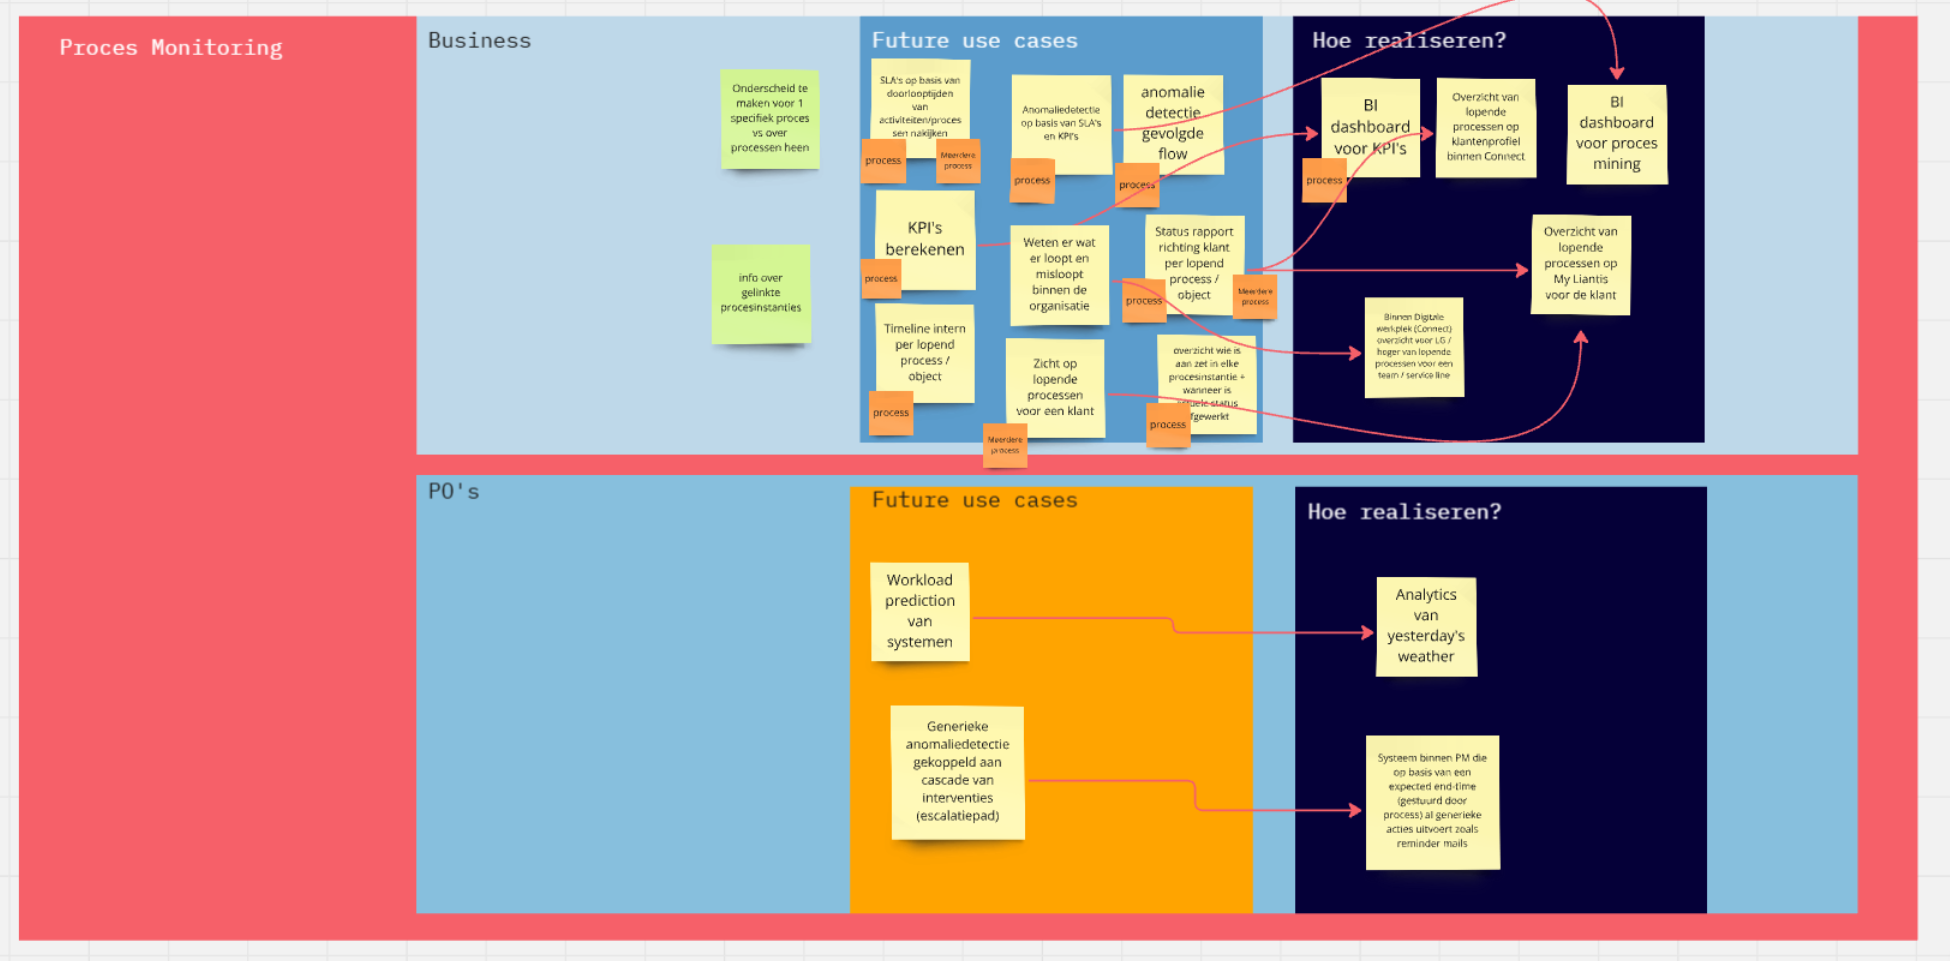
\includegraphics[width=1.0\linewidth]{PM.png}
  \captionof{figure}{Requirements Workshop}
  \vspace{0.5cm}
\end{center}

\begin{center}
  \captionsetup{type=figure}
  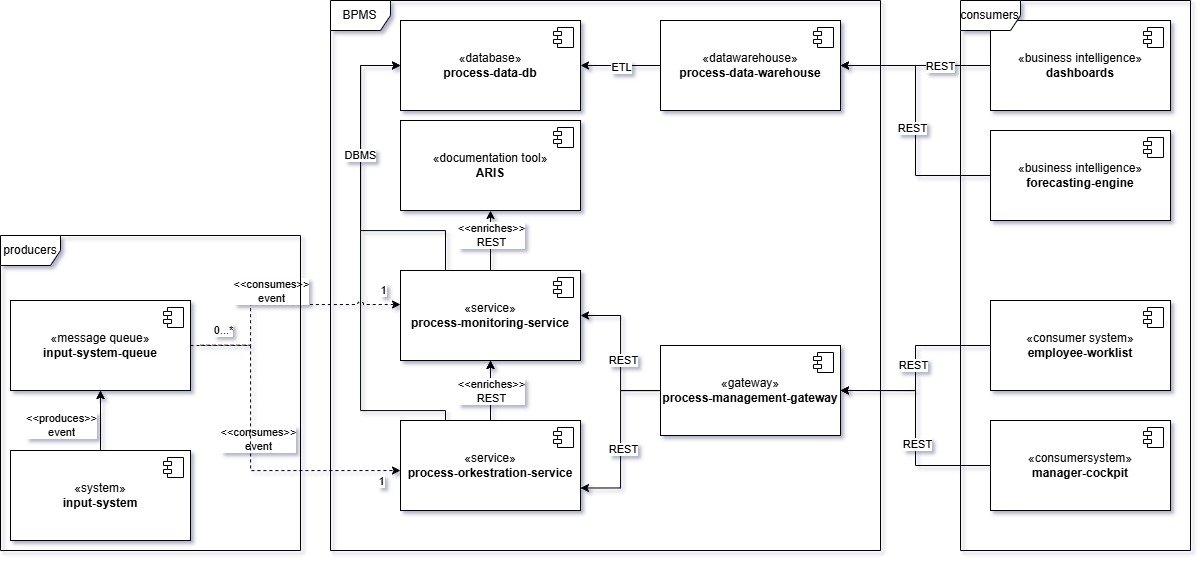
\includegraphics[width=1.0\linewidth]{theoretisch architectuur.jpg}
  \captionof{figure}{Design en Bouw van Proof-of-Concept}
  \vspace{0.5cm}
\end{center}

\begin{center}
  \captionsetup{type=figure}
  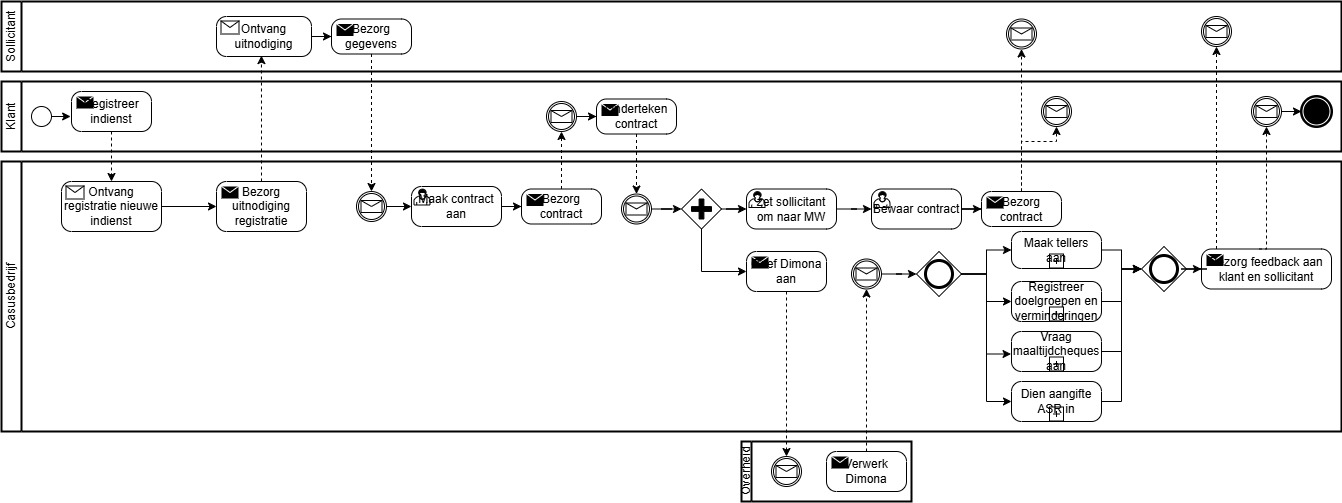
\includegraphics[width=1.0\linewidth]{test proces.jpg}
  \captionof{figure}{Simulatie van Proces}
  \vspace{0.5cm}
\end{center}

\begin{center}
  \captionsetup{type=figure}
  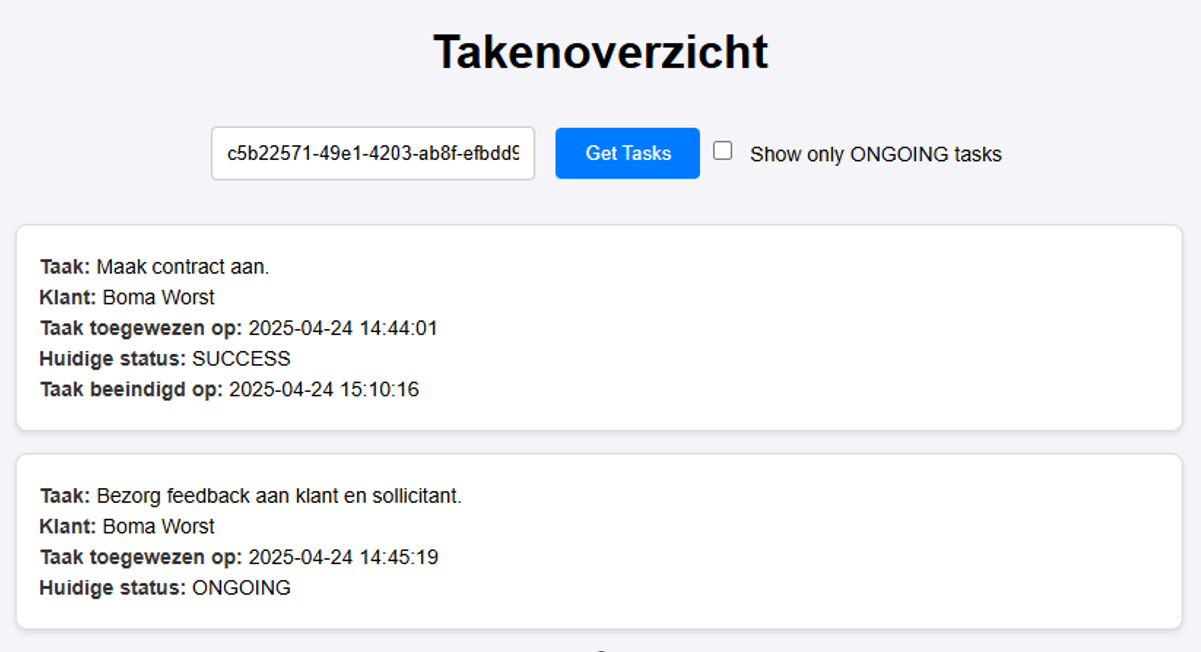
\includegraphics[width=1.0\linewidth]{takenoverzicht non-filtered.png}
  \captionof{figure}{Validatie en Visualisatie van Systeem}
  \vspace{0.5cm}
\end{center}
%==============================================================================
% Lower Right Column
%==============================================================================
\end{multicols}
\end{document}